\begin{frame}{Cuestión a abordar}
  \centering
  ¿Existe un algoritmo que para un conjunto dinámico, dado, de discos en
  el plano mantenga un conjunto independiente máximo aproximado de factor
  constante en tiempo de actualización poli-logarítmico?

  \begin{figure}  
    \centering
    
\includegraphics[width=0.6\textwidth]{./Images/autocuestionamiento.jpg}
  \end{figure}
\end{frame}


\begin{frame}{Ejecución}
  Supongamos el siguiente conjunto de discos unitarios en el plano
  \begin{figure}  
    \centering
    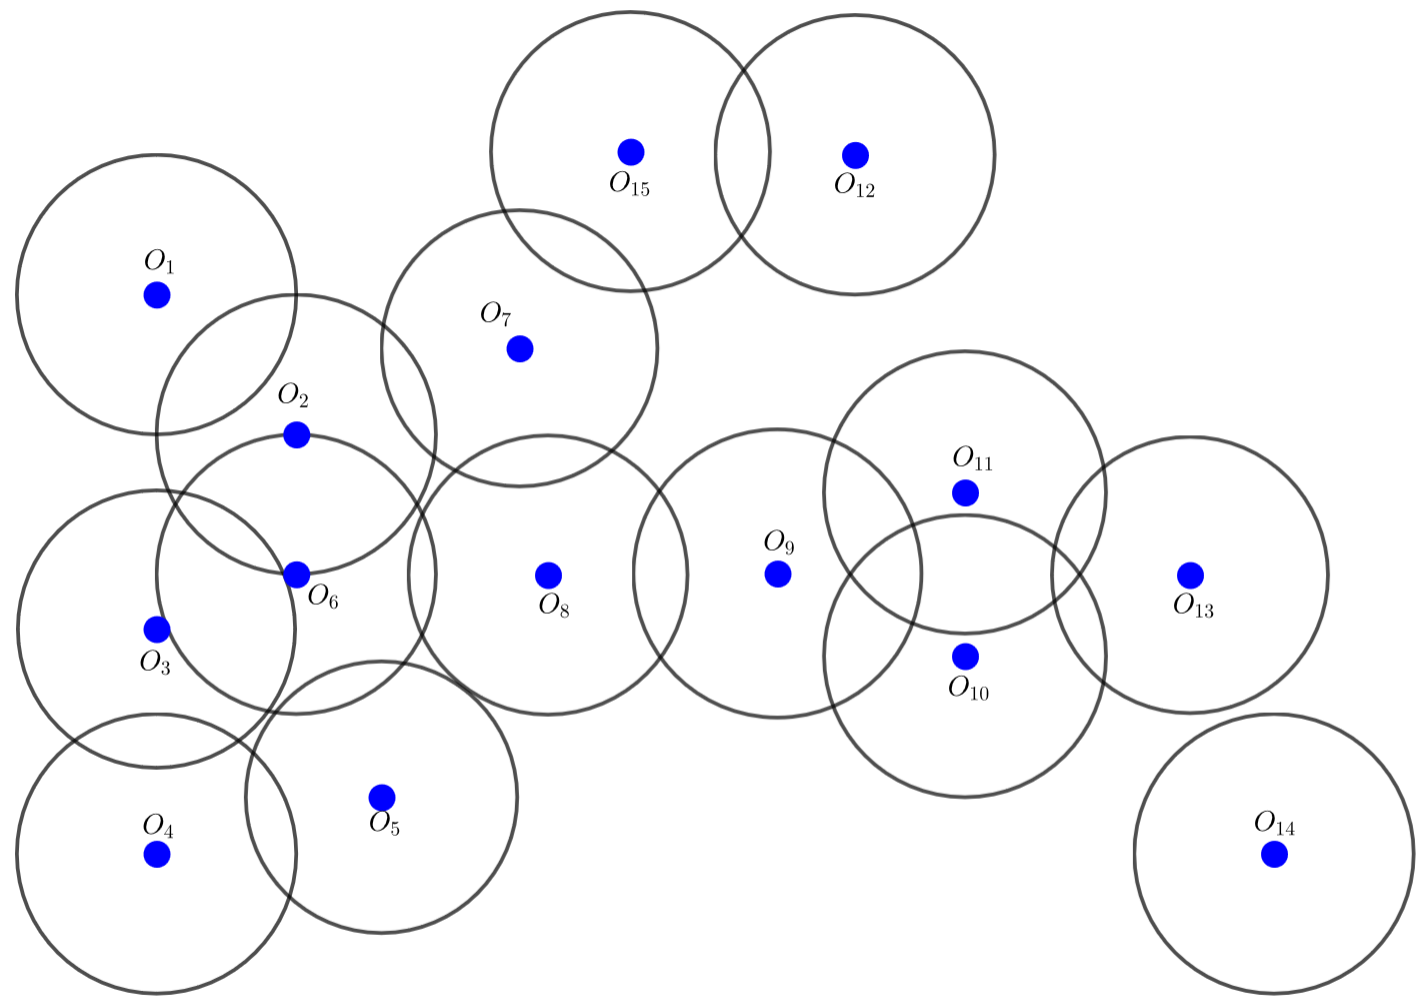
\includegraphics[width=0.8\textwidth]{./Images/01.png}
  \end{figure}
\end{frame}

\begin{frame}{...}
  Obtengamos su dualidad
  \begin{figure}  
    \centering
    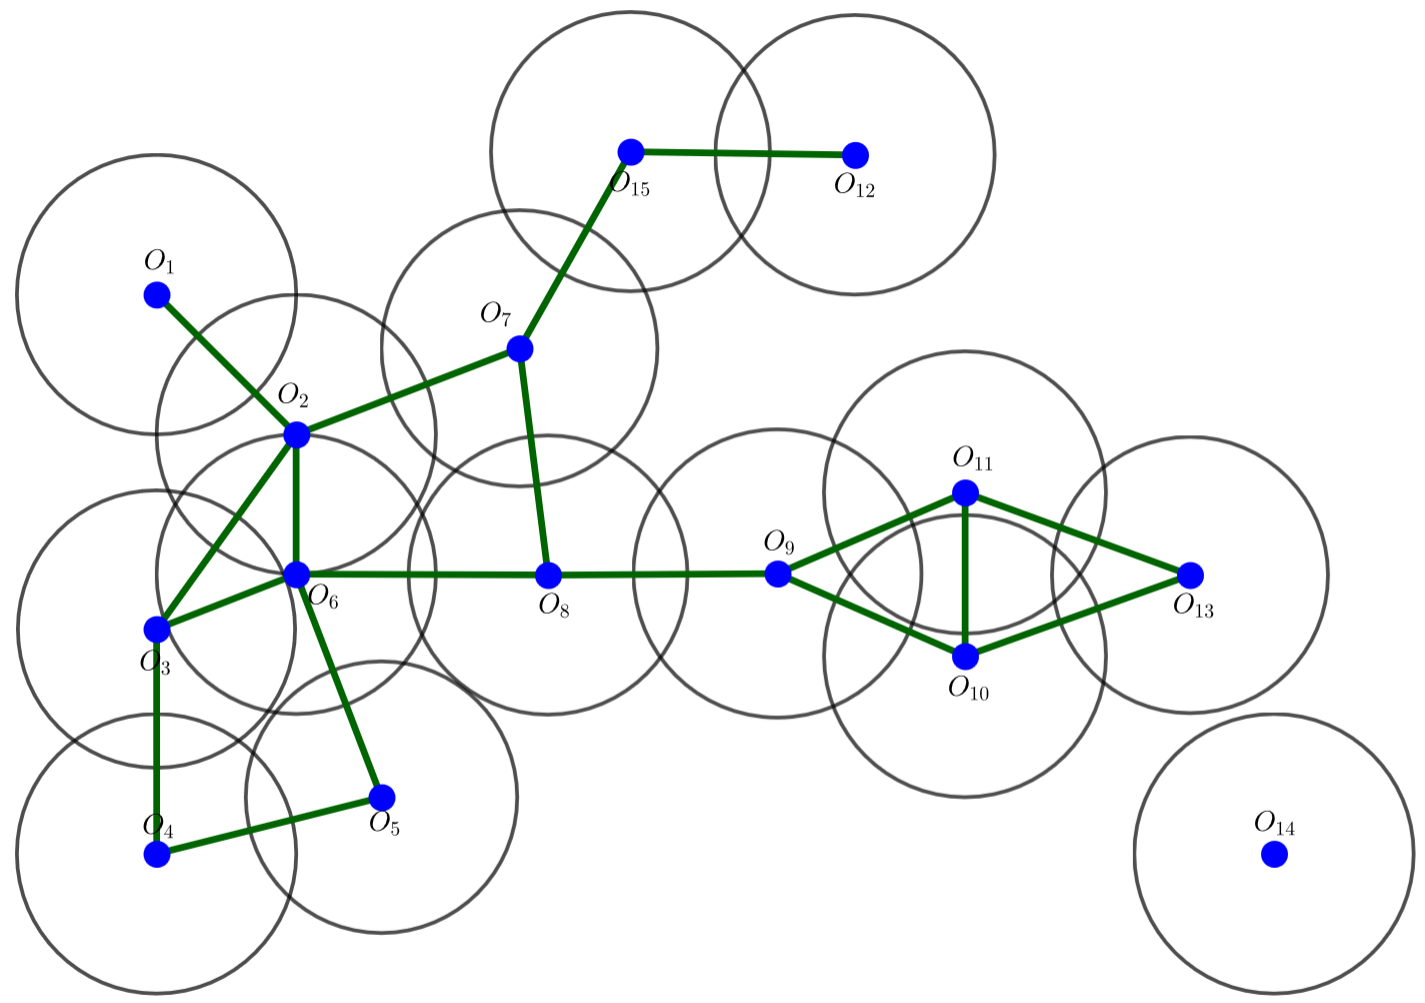
\includegraphics[width=0.8\textwidth]{./Images/02.png}
  \end{figure}
\end{frame}

\begin{frame}{...}
  Observemos su gráfica dual
  \begin{figure}  
    \centering
    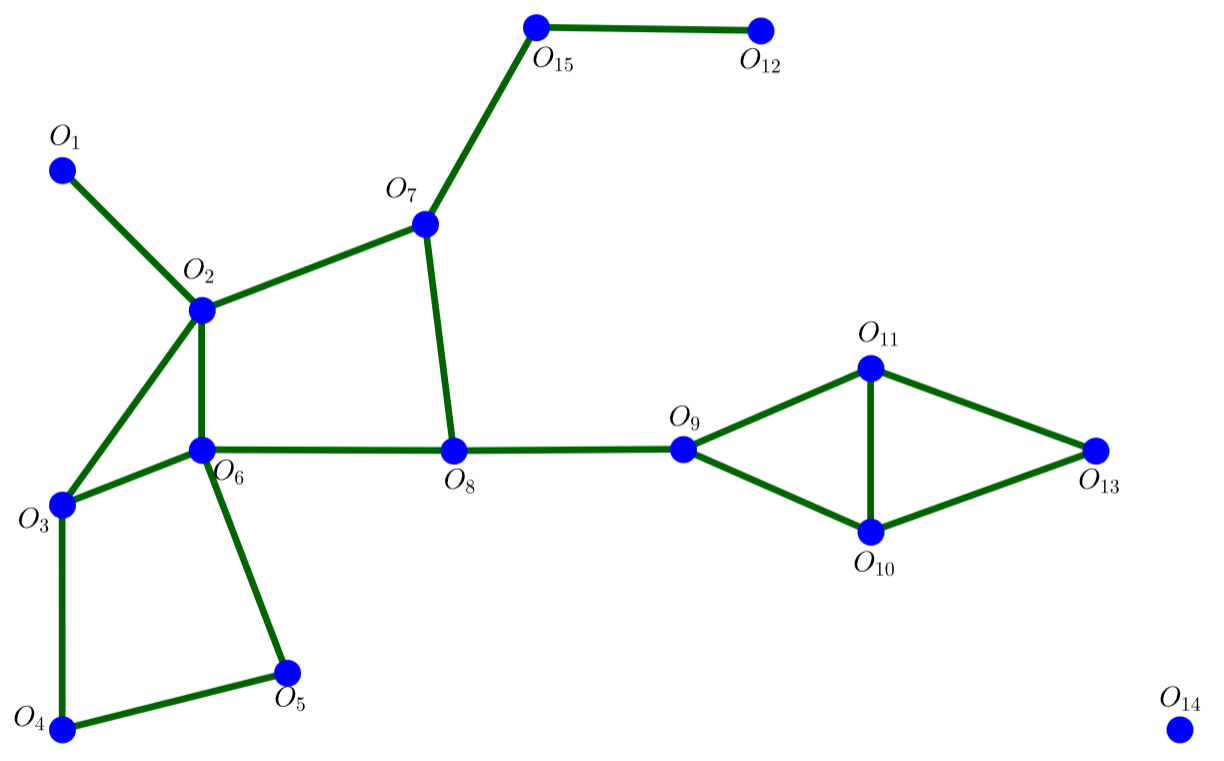
\includegraphics[width=0.8\textwidth]{./Images/SET.png}
  \end{figure}
  \textbf{Obs.} Existe un preprocesamiento que se encarga de exhibir candidatos a OPT.
\end{frame}

\begin{frame}{...}
  Sea $S_1 = \{O_1, O_6, O_4, O_7, O_{12}, O_9, O_{13}, O_{14}\}$
  \begin{figure}  
    \centering
    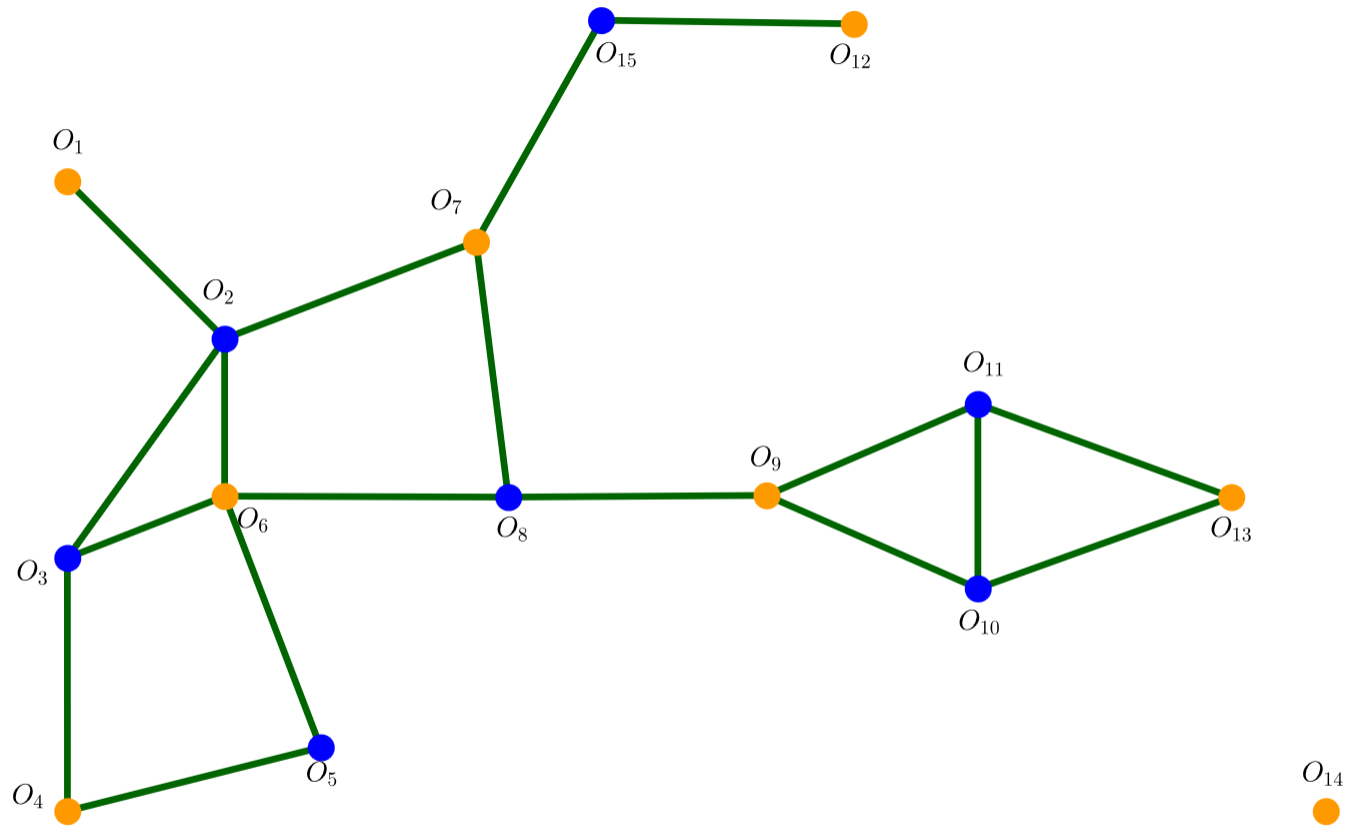
\includegraphics[width=0.8\textwidth]{./Images/S1.png}
  \end{figure}
\end{frame}

\begin{frame}{...}
  Sea $S_2 = \{O_2, O_4, O_8, O_{15}, O_{11}, O_{14}\}$
  \begin{figure}  
    \centering
    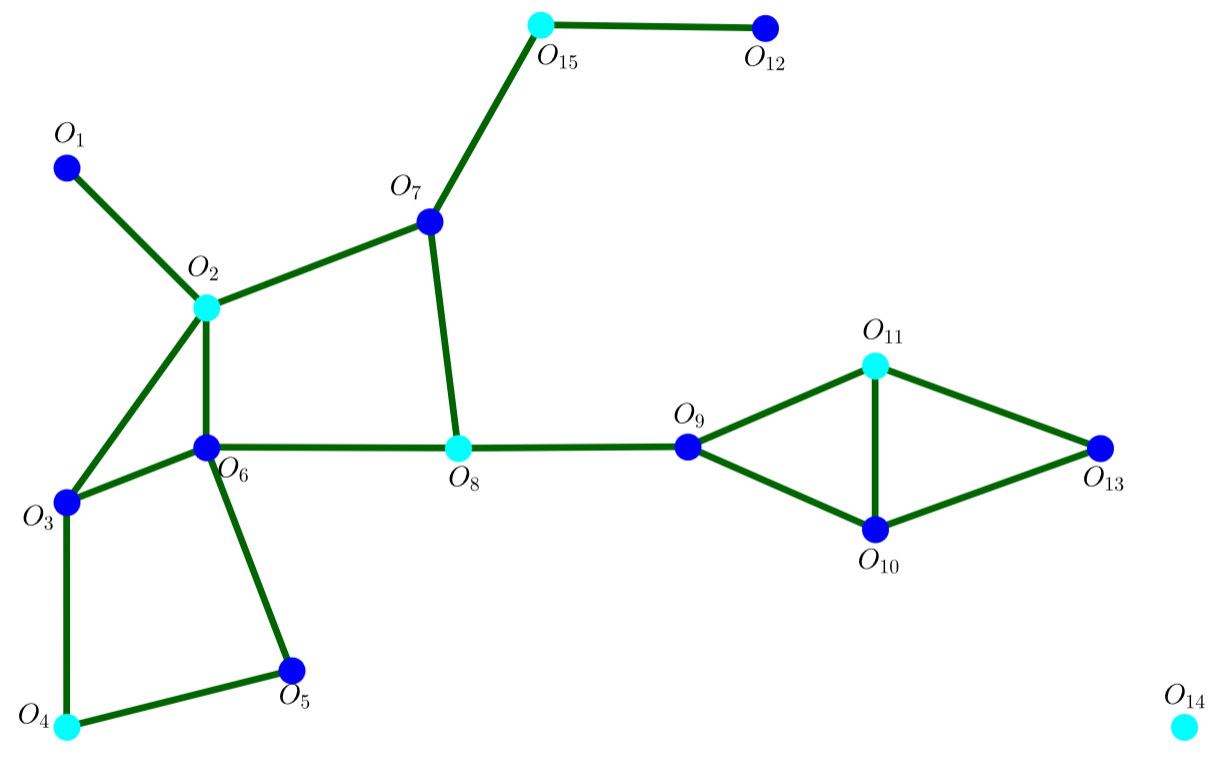
\includegraphics[width=0.8\textwidth]{./Images/S2.png}
  \end{figure}
\end{frame}


\begin{frame}{...}
  Sea $S_3 = \{O_1, O_3, O_5, O_7, O_{12}, O_{9}, O_{13}, O_{14}\}$
  \begin{figure}  
    \centering
    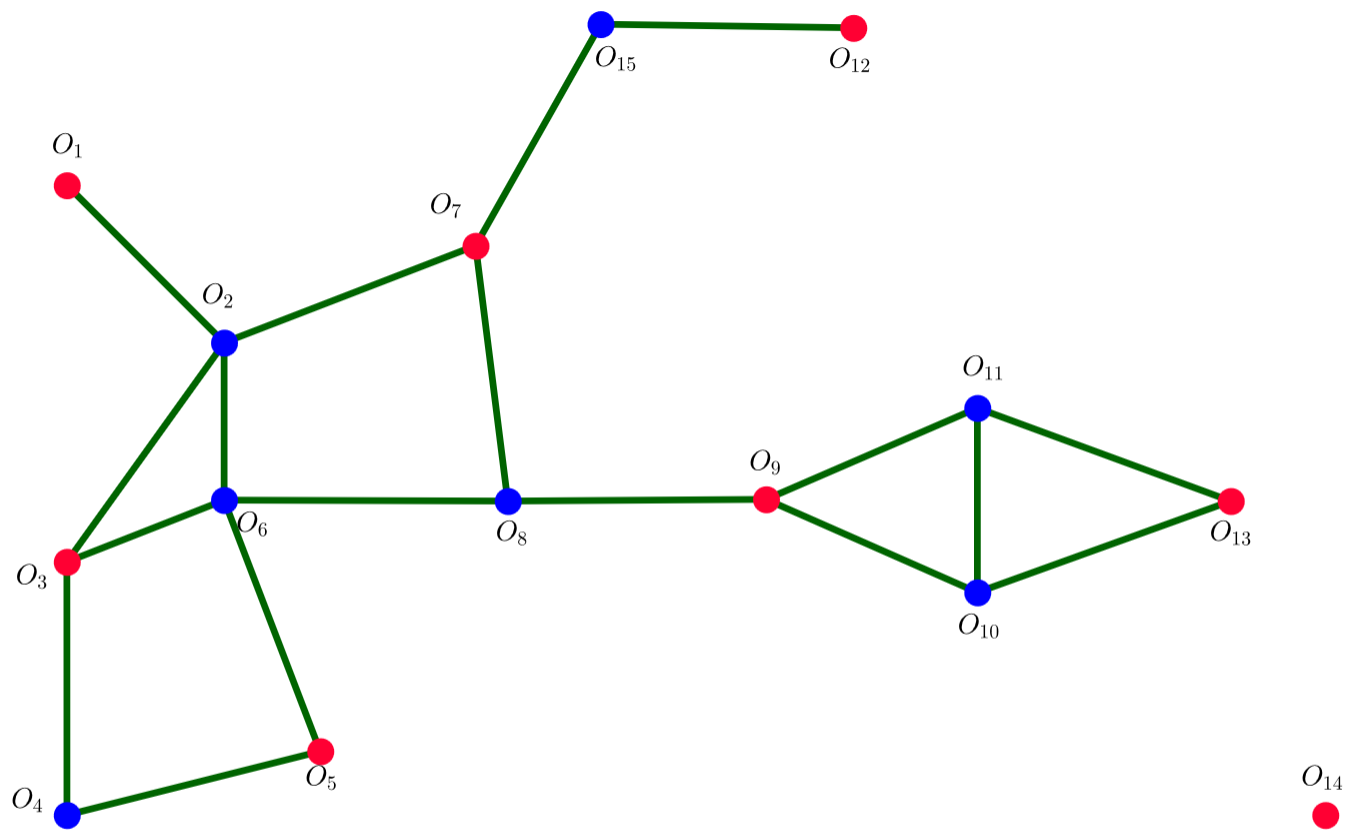
\includegraphics[width=0.8\textwidth]{./Images/S3.png}
  \end{figure}
\end{frame}

\begin{frame}{...}
  Sea $S_{MIS} = \{S_1, S_2, S_3\}$. Elijamos un candidato de $S_{MIS}$ tal que sea de mayor tamaño,
  digamos $S = S_1$. Ahora, eliminemos $O_{13}$.
  \begin{figure}  
    \centering
    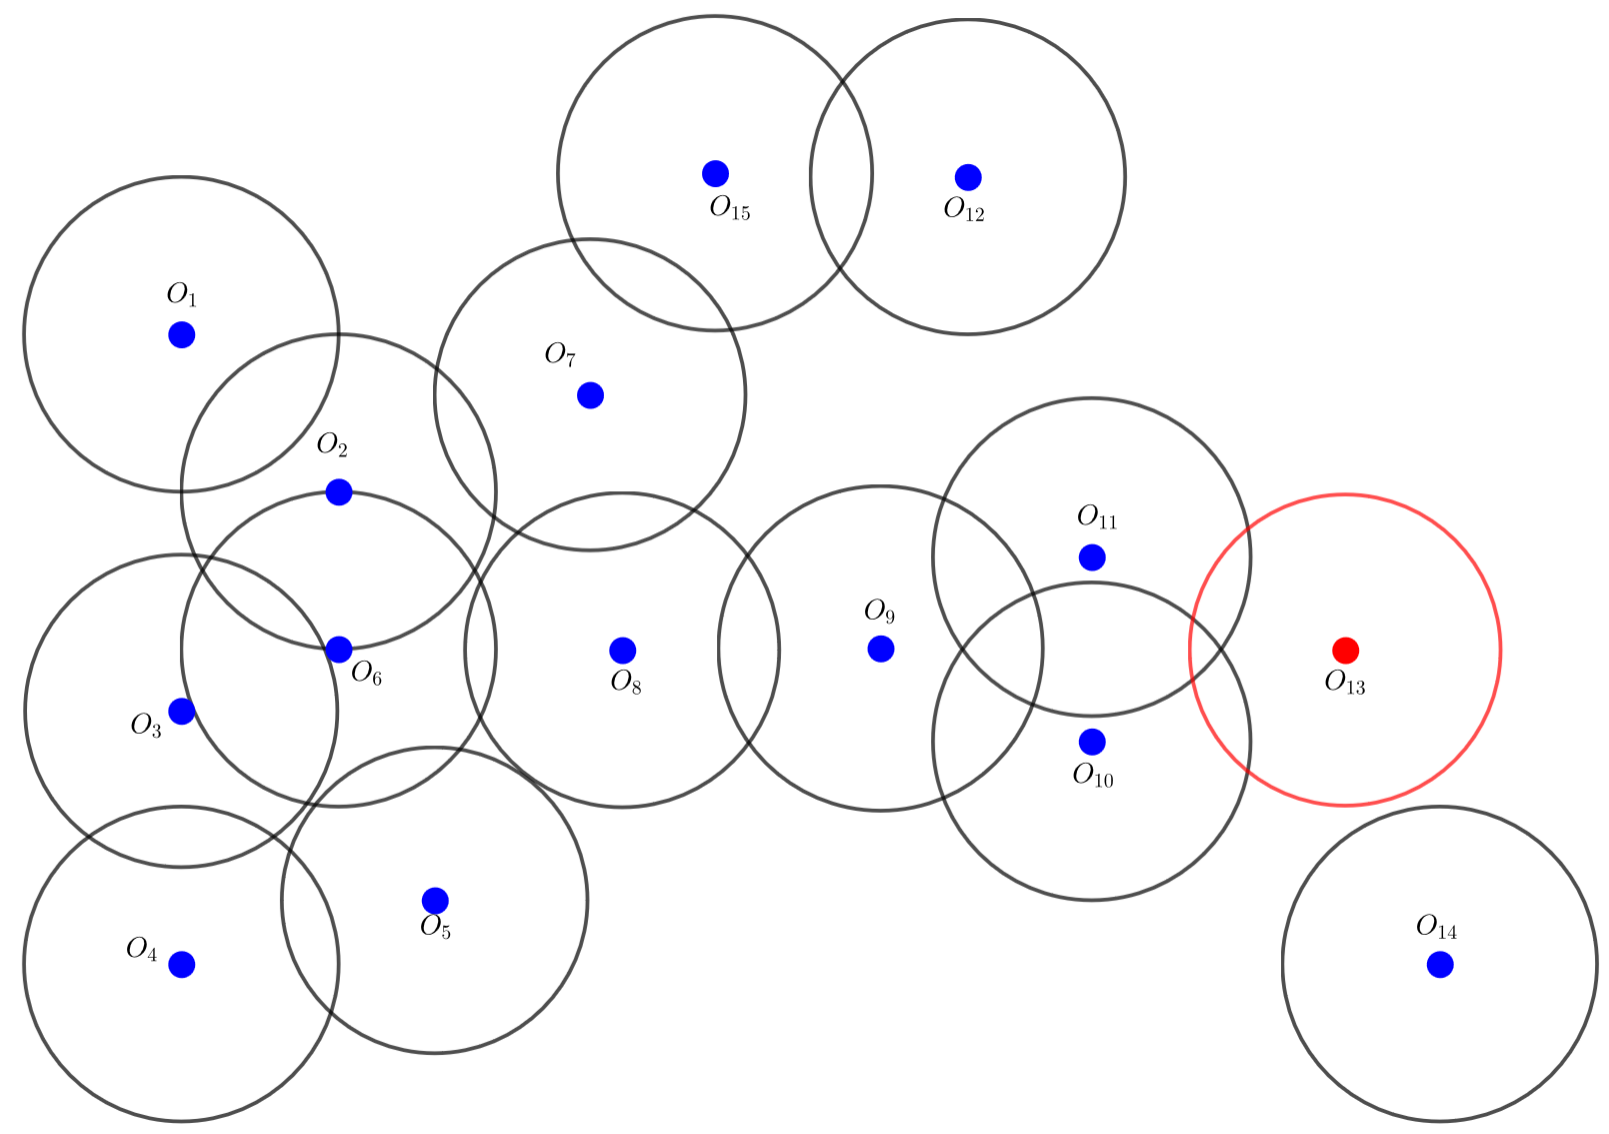
\includegraphics[width=0.8\textwidth]{./Images/03.png}
  \end{figure}
\end{frame}

\begin{frame}{...}
  Cómo hemos hecho una eliminación, debemos actualizar $S_1 = S_1/O_{13}$,
  $S_2 = S_2/O_{13}$, $S_3 = S_3/O_{13}$.
  \begin{figure}  
    \centering
    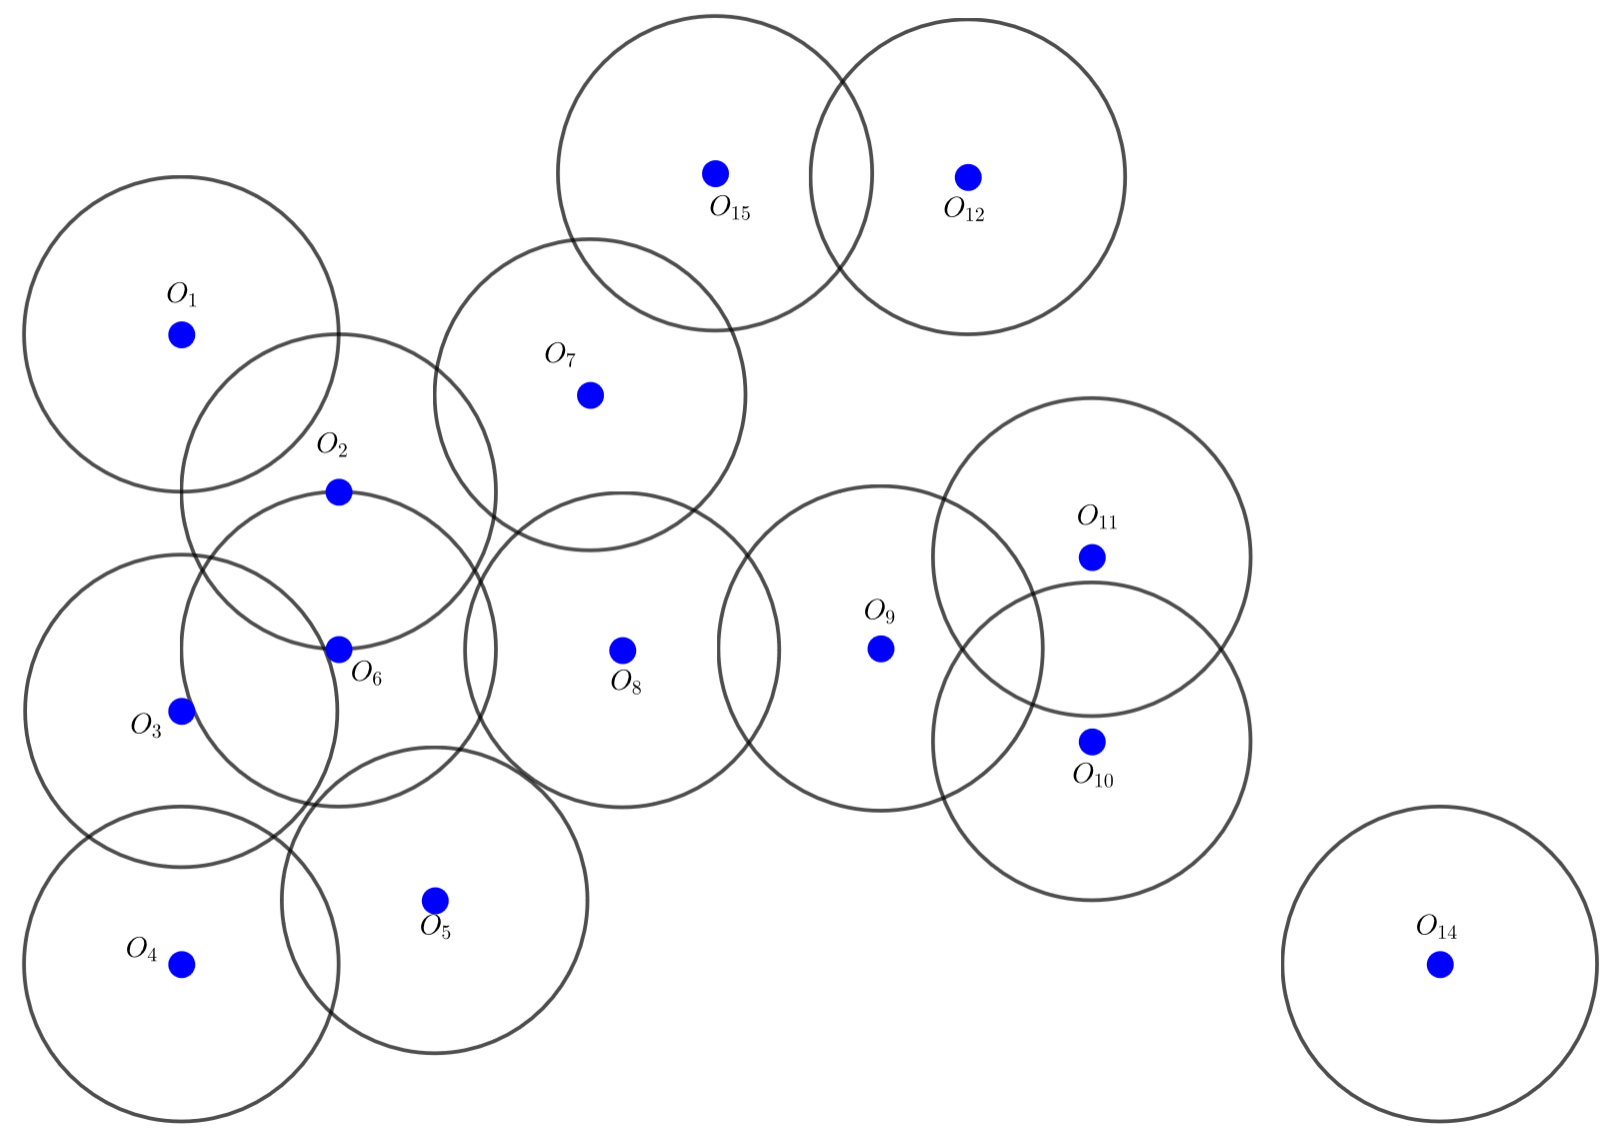
\includegraphics[width=0.8\textwidth]{./Images/04.png}
  \end{figure}
  $S = \{O_1, O_6, O_4, O_7, O_{12}, O_9, O_{14}\}$.
\end{frame}

\begin{frame}{...}
  Añadamos $O_{13}$ (un nuevo disco)
  \begin{figure}  
    \centering
    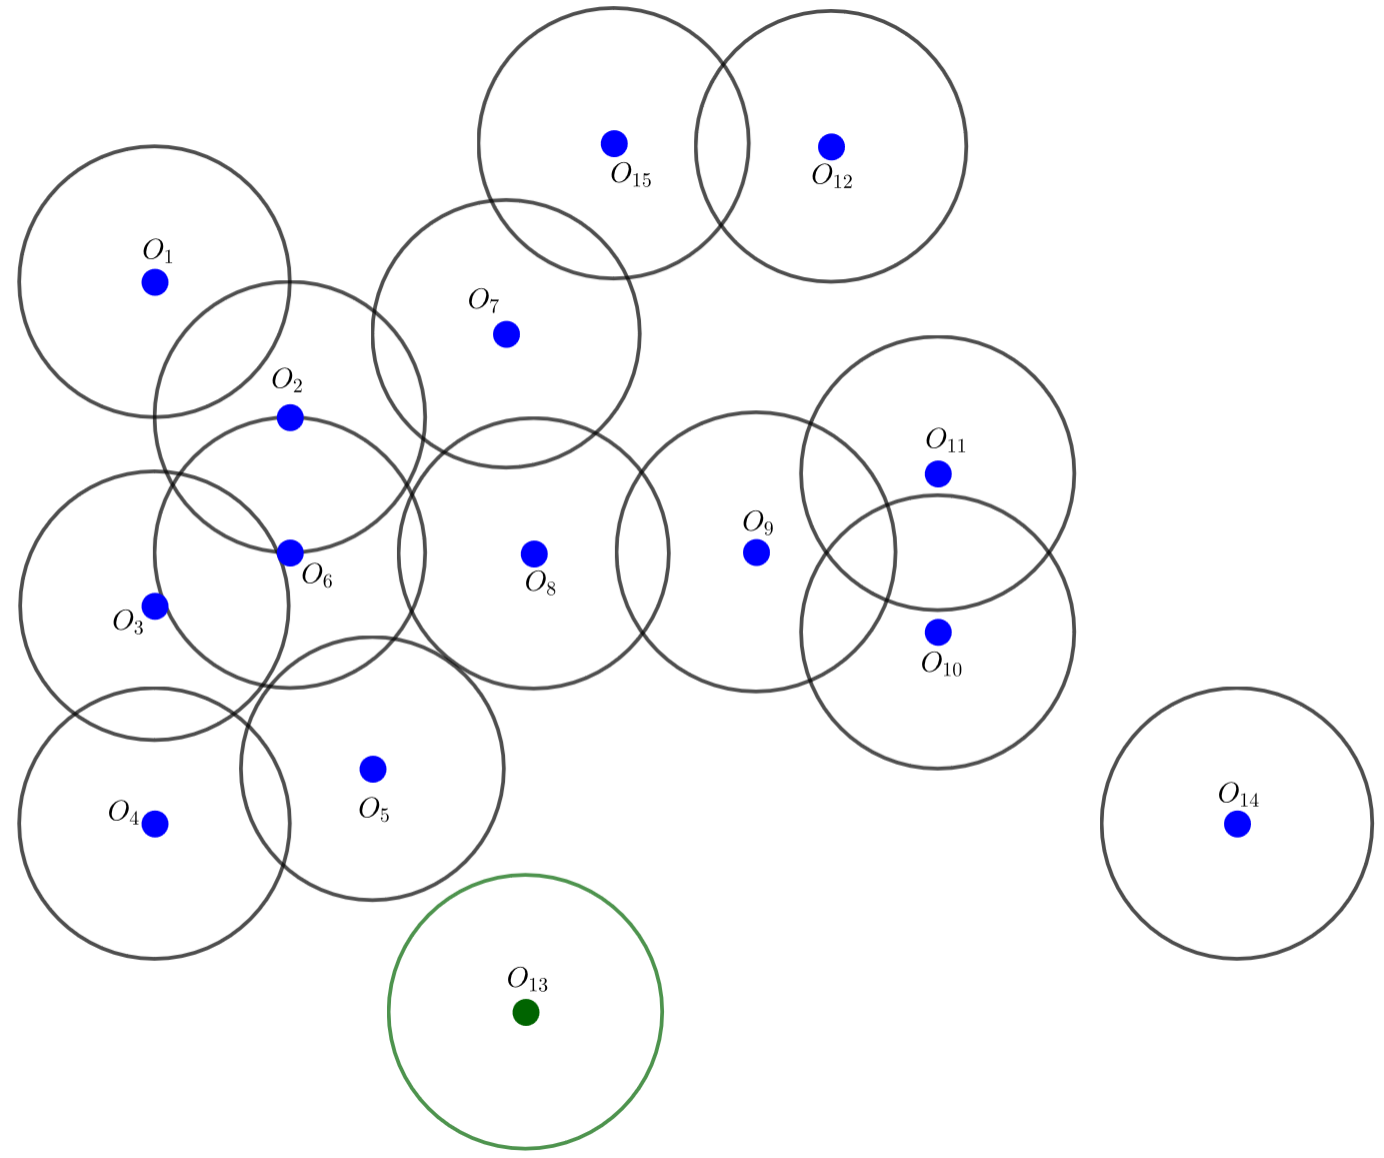
\includegraphics[width=0.7\textwidth]{./Images/05.png}
  \end{figure}

\end{frame}

\begin{frame}{...}
  Verificamos si este disco debe formar parte de los candidatos,
  en este caso actualizamos $S_1 = S_1 \cup \{O_{13}\}$, $S_2 = S_2 \cup \{O_{13}\}$,
  $S_3 = S_3 \cup \{O_{13}\}$. Y  $S = \{O_1, O_6, O_4, O_7, O_{12}, O_{13}, O_9, O_{14}\}$.
  \begin{figure}  
    \centering
    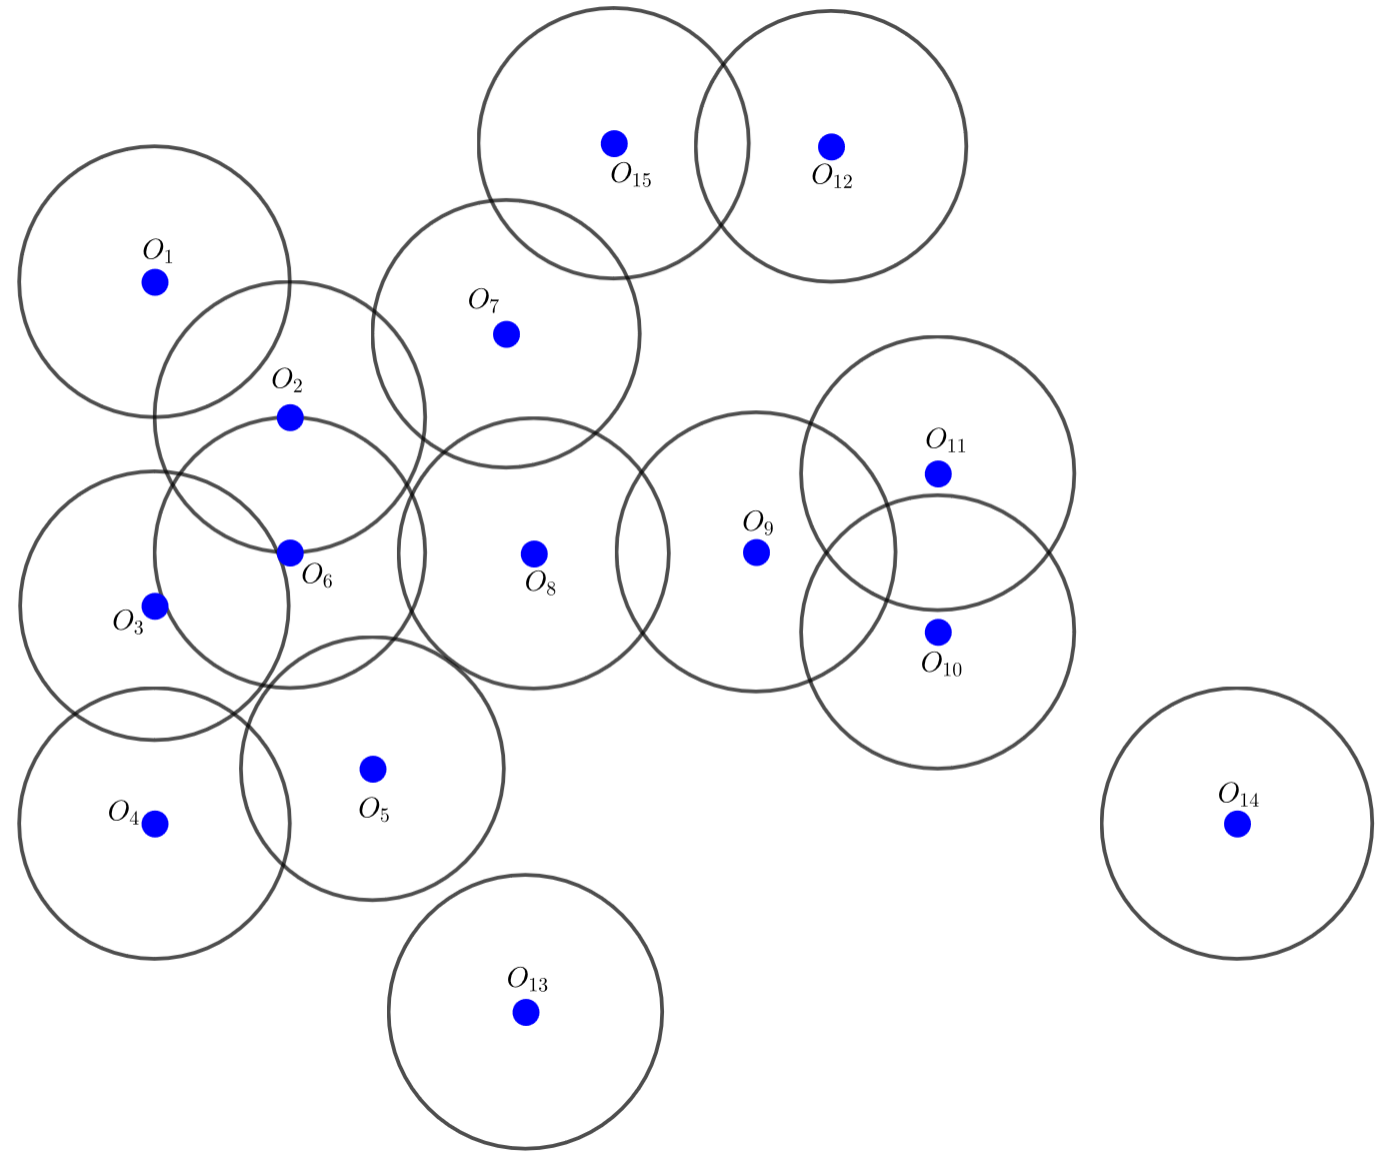
\includegraphics[width=0.7\textwidth]{./Images/06.png}
  \end{figure}
\end{frame}

\begin{frame}{...}
  Eliminemos $O_{15}$
  \begin{figure}  
    \centering
    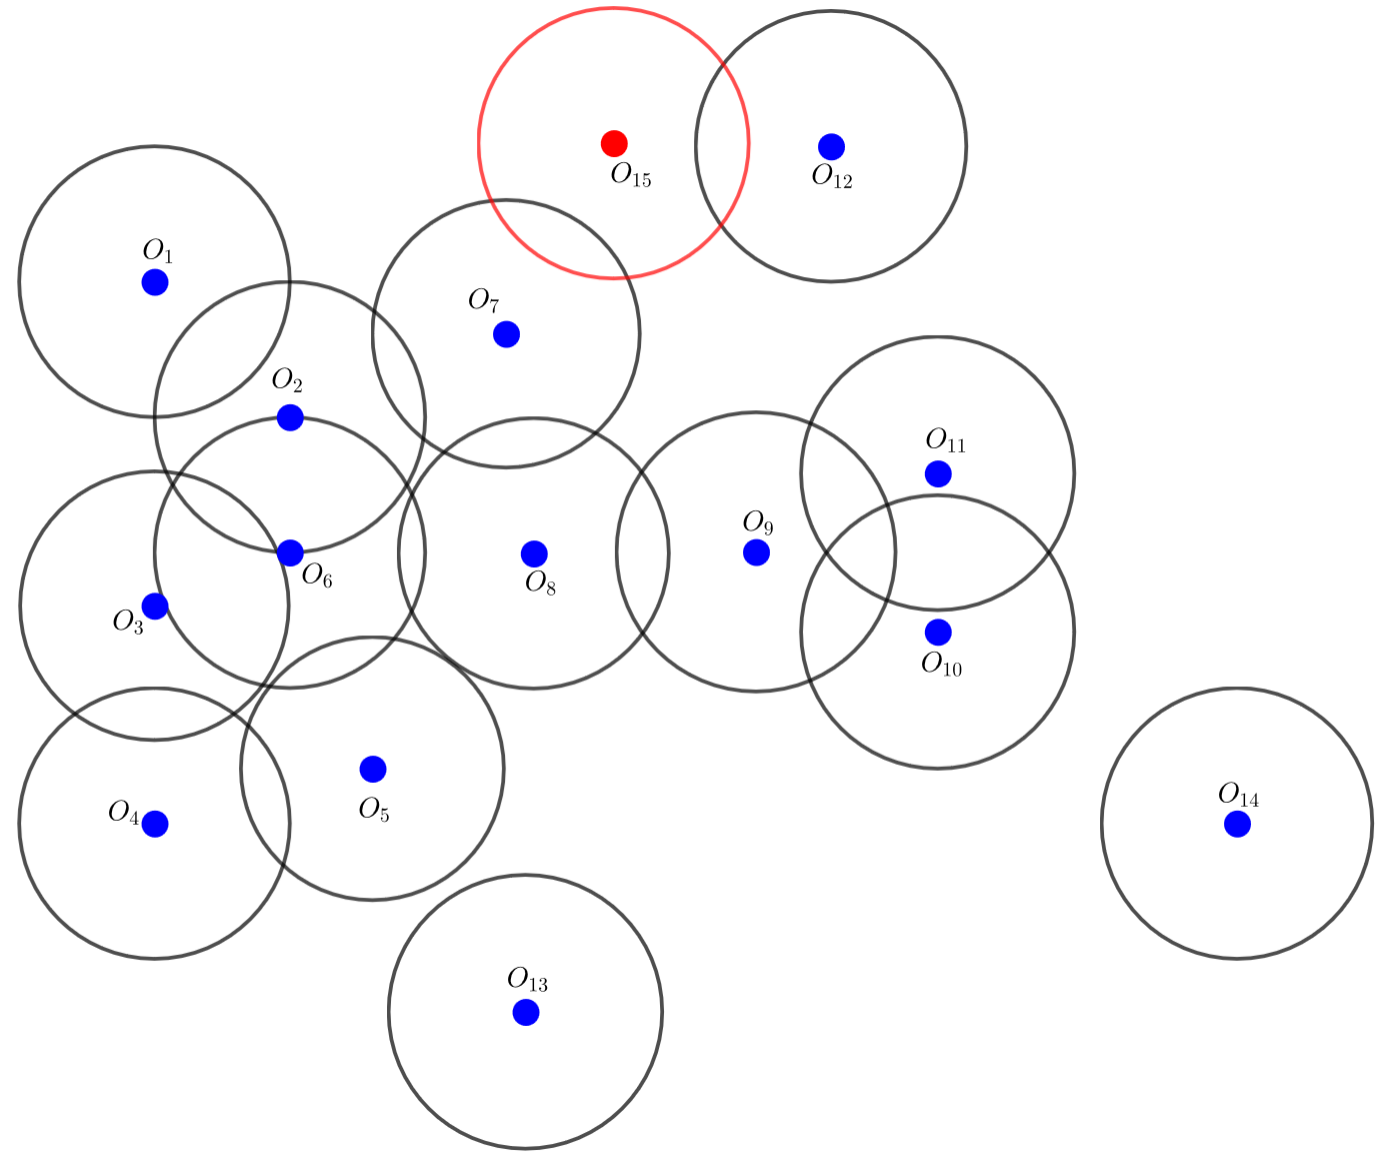
\includegraphics[width=0.7\textwidth]{./Images/07.png}
  \end{figure}
\end{frame}

\begin{frame}{...}
  Verificamos si está eliminación afecta a nuestros candidatos, en este caso
  no se ven afectados y continuamos
  \begin{figure}  
    \centering
    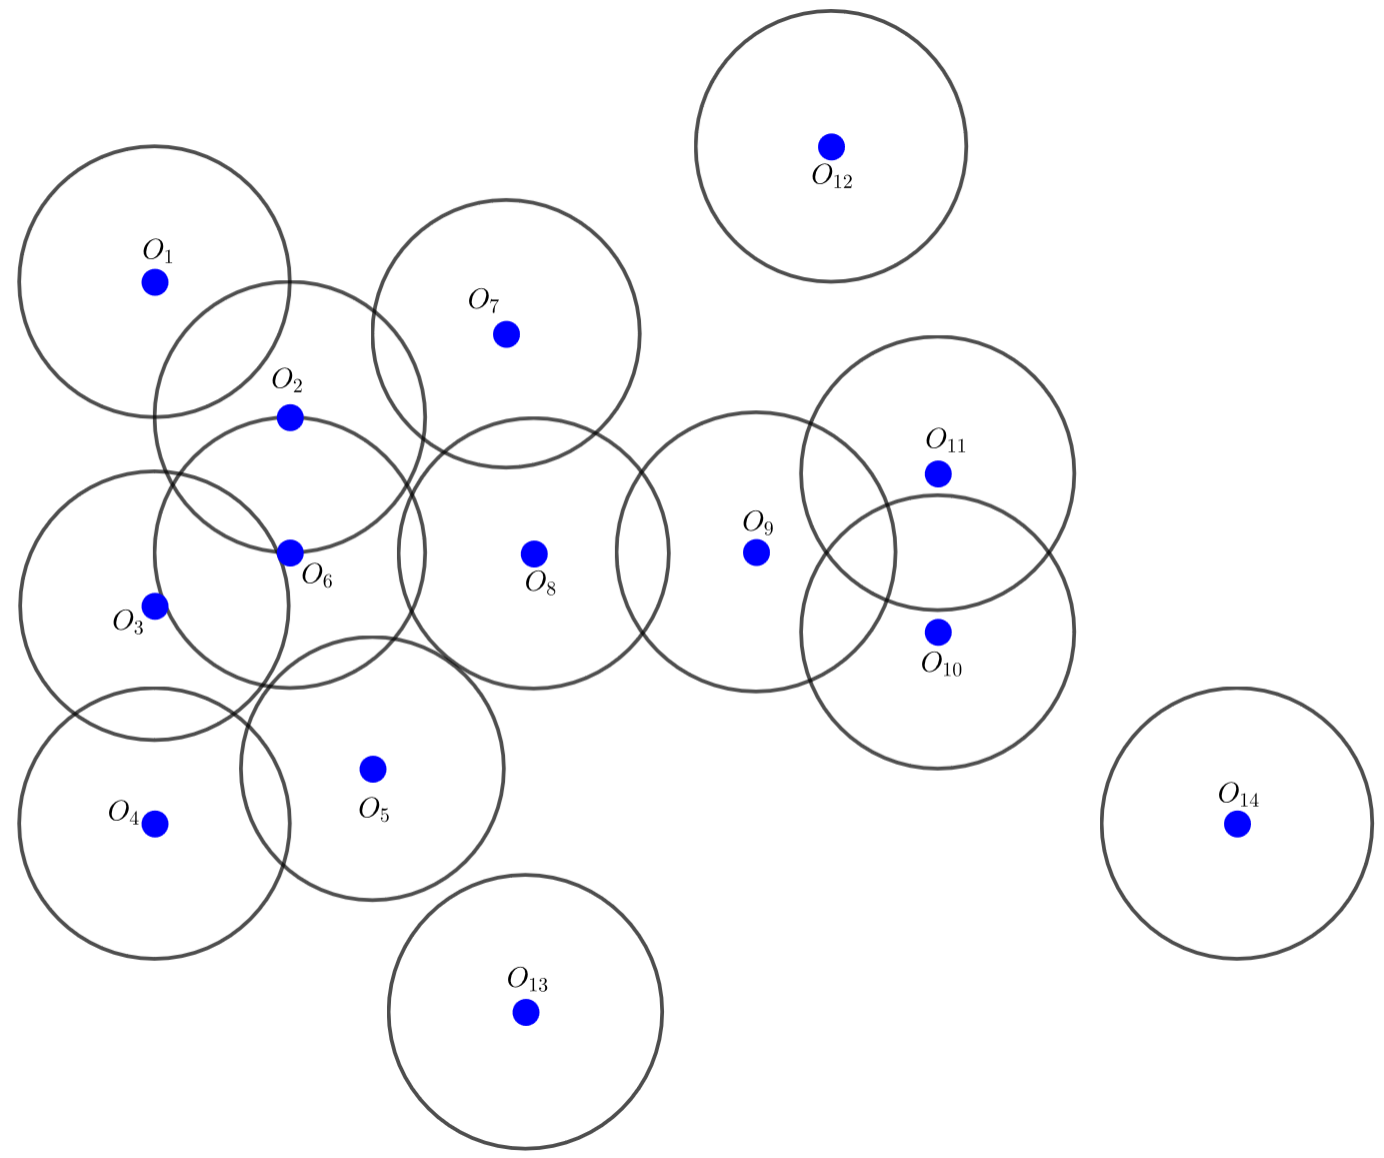
\includegraphics[width=0.7\textwidth]{./Images/08.png}
  \end{figure}
  $S = \{O_1, O_6, O_4, O_7, O_{12}, O_{13}, O_9, O_{14}\}$
\end{frame}

\begin{frame}{...}
  Eliminamos $O_{14}$
  \begin{figure}  
    \centering
    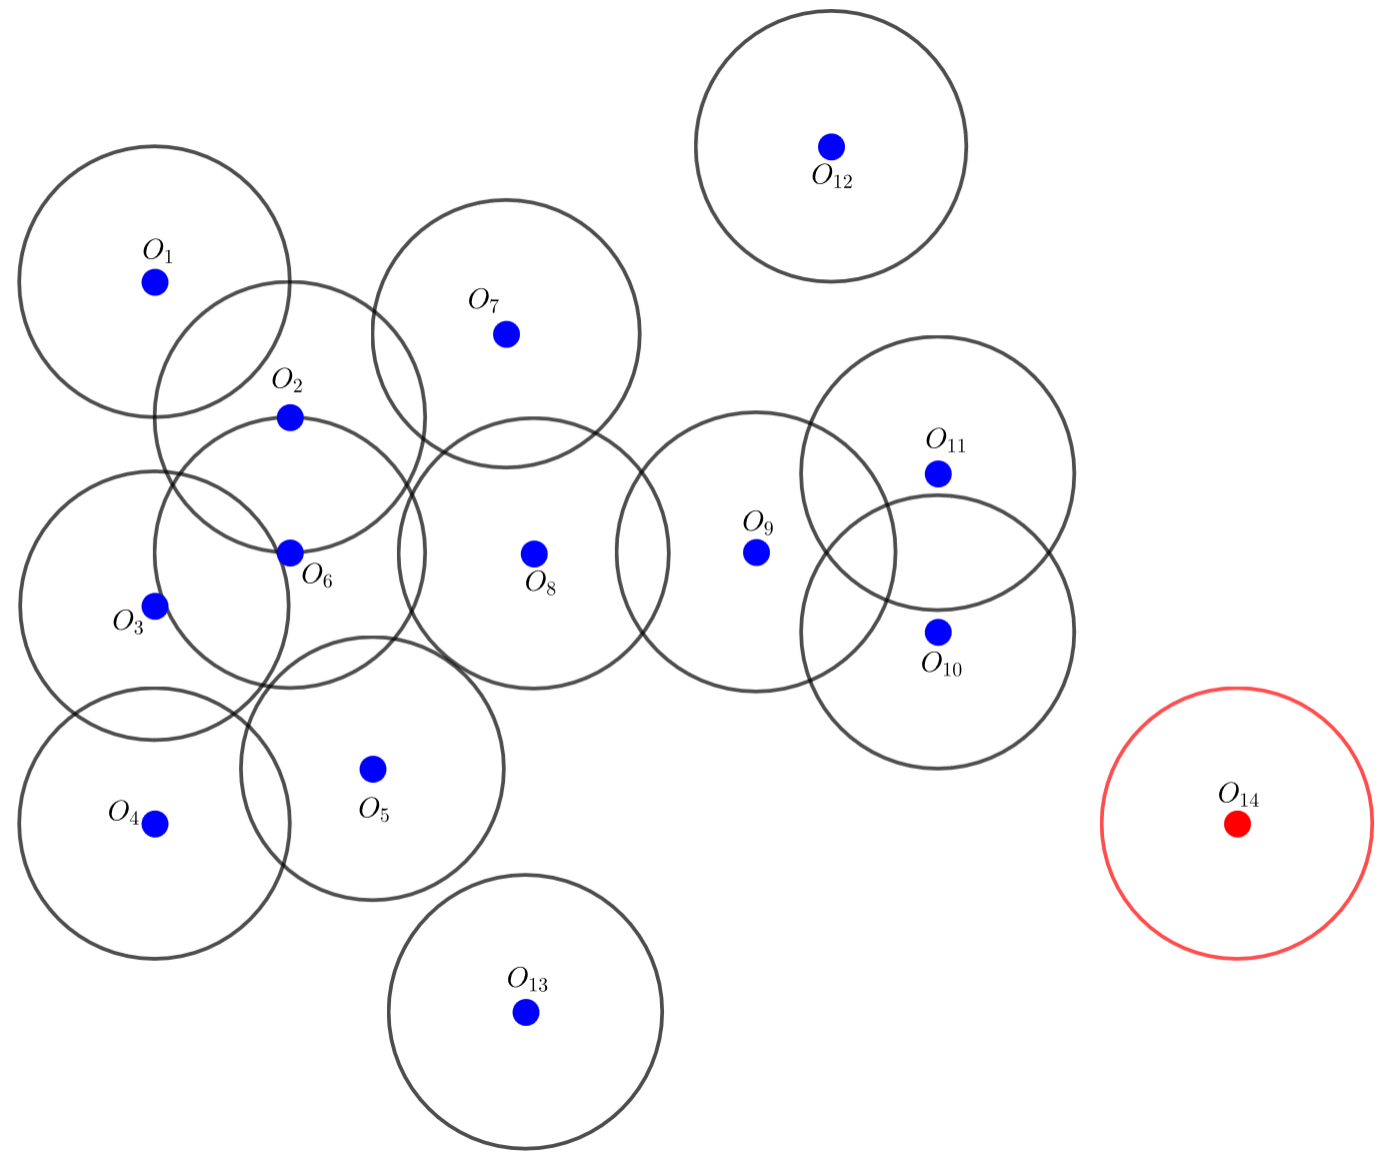
\includegraphics[width=0.7\textwidth]{./Images/09.png}
  \end{figure}
  
\end{frame}

\begin{frame}{...}
  Actualizamos los estados de nuestros candidatos $S_1 = S_1/O_{14}$,
  $S_2 = S_2/O_{14}$, $S_3 = S_3/O_{14}$.
  \begin{figure}  
    \centering
    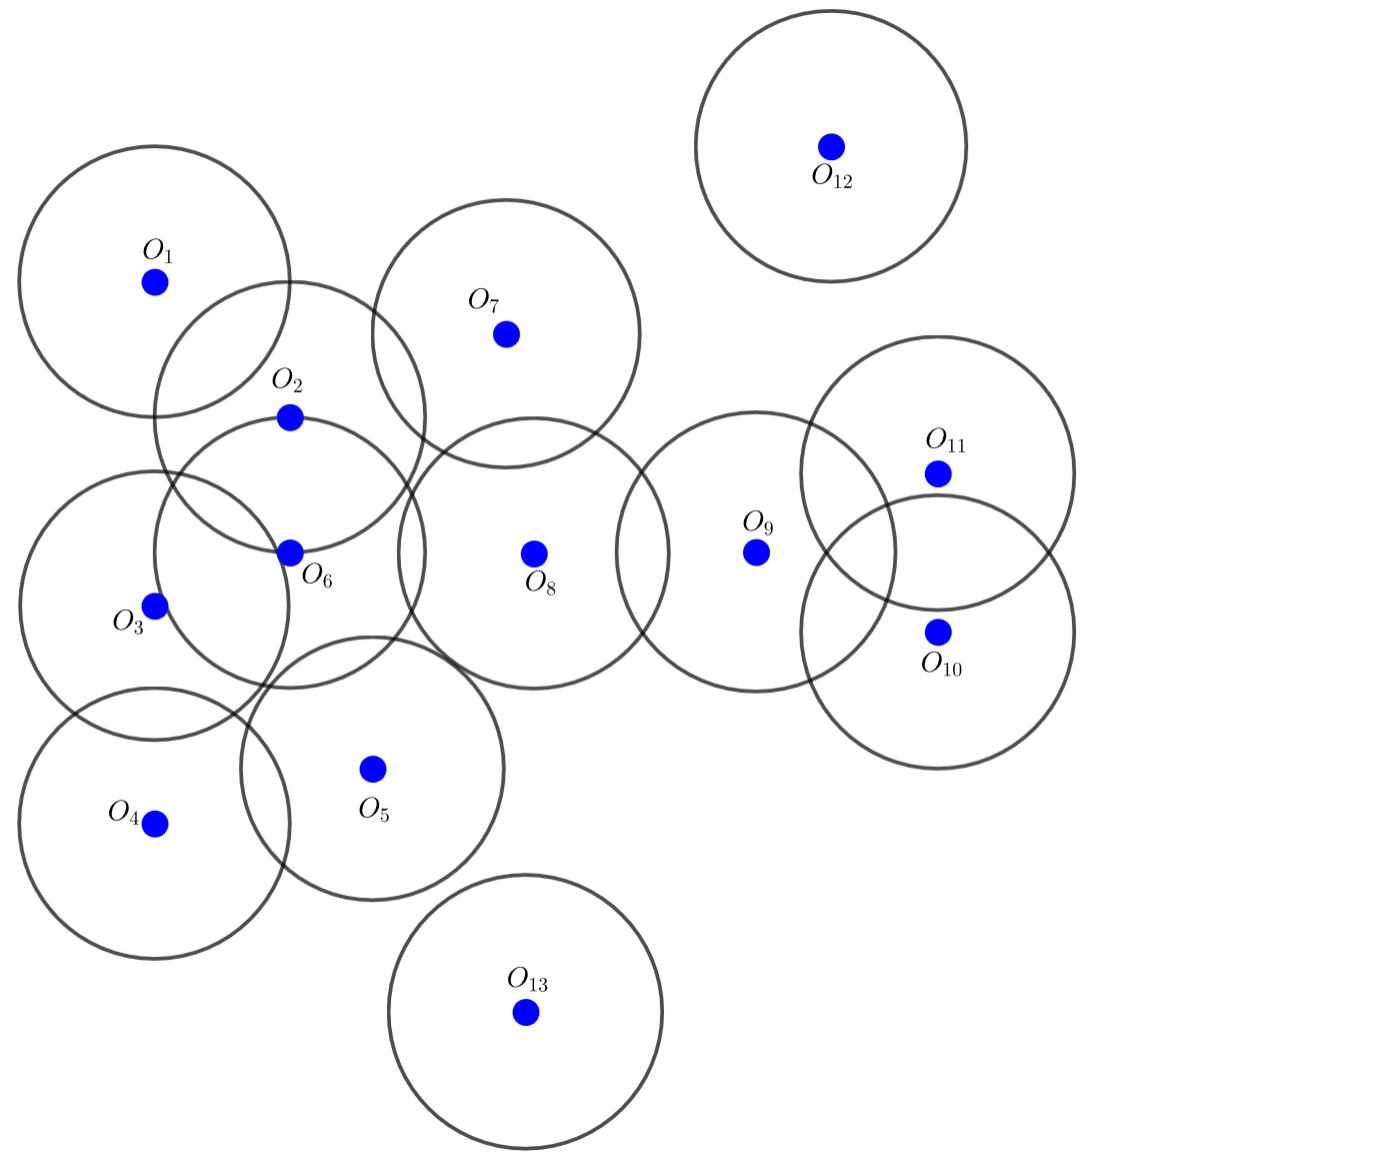
\includegraphics[width=0.7\textwidth]{./Images/10.png}
  \end{figure}
    $S = \{O_1, O_6, O_4, O_7, O_{12}, O_{13}, O_9\}$. \textbf{FIN.}
\end{frame}
